\documentclass{beamer}
\usepackage{amsmath}
\usepackage[english]{babel} %set language; note: after changing this, you need to delete all auxiliary files to recompile
\usepackage[utf8]{inputenc} %define file encoding; latin1 is the other often used option
\usepackage{csquotes} % provides context sensitive quotation facilities
\usepackage{graphicx} %allows for inserting figures
\usepackage{booktabs} % for table formatting without vertical lines
\usepackage{textcomp} % allow for example using the Euro sign with \texteuro
\usepackage{stackengine}
\usepackage{wasysym}
\usepackage{tikzsymbols}
\usepackage{textcomp}
\usetikzlibrary{patterns} 
\usepackage{xcolor}
\usepackage[dvipsnames]{xcolor}
\usepackage{colortbl}
\usepackage{adjustbox}
\usetikzlibrary{decorations}
\usetikzlibrary{decorations.pathreplacing}
\usetikzlibrary{decorations.markings}
\newcommand{\bubblethis}[2]{
        \tikz[remember picture,baseline]{\node[anchor=base,inner sep=0,outer sep=0]%
        (#1) {\underline{#1}};\node[overlay,cloud callout,callout relative pointer={(0.2cm,-0.7cm)},%
        aspect=2.5,fill=yellow!90] at ($(#1.north)+(-0.5cm,1.6cm)$) {#2};}%
    }%
\tikzset{face/.style={shape=circle,minimum size=4ex,shading=radial,outer sep=0pt,
        inner color=white!50!yellow,outer color= yellow!70!orange}}
%% Some commands to make the code easier
\newcommand{\emoticon}[1][]{%
  \node[face,#1] (emoticon) {};
  %% The eyes are fixed.
  \draw[fill=white] (-1ex,0ex) ..controls (-0.5ex,0.2ex)and(0.5ex,0.2ex)..
        (1ex,0.0ex) ..controls ( 1.5ex,1.5ex)and( 0.2ex,1.7ex)..
        (0ex,0.4ex) ..controls (-0.2ex,1.7ex)and(-1.5ex,1.5ex)..
        (-1ex,0ex)--cycle;}
\newcommand{\pupils}{
  %% standard pupils
  \fill[shift={(0.5ex,0.5ex)},rotate=80] 
       (0,0) ellipse (0.3ex and 0.15ex);
  \fill[shift={(-0.5ex,0.5ex)},rotate=100] 
       (0,0) ellipse (0.3ex and 0.15ex);}

\newcommand{\emoticonname}[1]{
  \node[below=1ex of emoticon,font=\footnotesize,
        minimum width=4cm]{#1};}
\usepackage{scalerel}
\usetikzlibrary{positioning}
\usepackage{xcolor,amssymb}
\newcommand\dangersignb[1][2ex]{%
  \scaleto{\stackengine{0.3pt}{\scalebox{1.1}[.9]{%
  \color{red}$\blacktriangle$}}{\tiny\bfseries !}{O}{c}{F}{F}{L}}{#1}%
}
\newcommand\dangersignw[1][2ex]{%
  \scaleto{\stackengine{0.3pt}{\scalebox{1.1}[.9]{%
  \color{red}$\blacktriangle$}}{\color{white}\tiny\bfseries !}{O}{c}{F}{F}{L}}{#1}%
}
\usepackage{fontawesome} % Social Icons
\usepackage{epstopdf} % allow embedding eps-figures
\usepackage{tikz} % allows drawing figures
\usepackage{amsmath,amssymb,amsthm} %advanced math facilities
\usepackage{lmodern} %uses font that support italic and bold at the same time
\usepackage{hyperref}
\usepackage{tikz}

\usepackage{tcolorbox}

\usefonttheme[onlymath]{serif} %set math font to serif ones

\definecolor{beamerblue}{rgb}{0.2,0.2,0.7} %define beamerblue color for later use

%%% defines highlight command to set text blue
\newcommand{\highlight}[1]{{\color{blue}{#1}}}


%%%%%%% commands defining backup slides so that frame numbering is correct

\newcommand{\backupbegin}{
   \newcounter{framenumberappendix}
   \setcounter{framenumberappendix}{\value{framenumber}}
}
\newcommand{\backupend}{
   \addtocounter{framenumberappendix}{-\value{framenumber}}
   \addtocounter{framenumber}{\value{framenumberappendix}}
}

%%%% end of defining backup slides

%Specify figure caption, see also http://tex.stackexchange.com/questions/155738/caption-package-not-working-with-beamer
\setbeamertemplate{caption}{\insertcaption} %redefines caption to remove label "Figure".
%\setbeamerfont{caption}{size=\scriptsize,shape=\itshape,series=\bfseries} %sets figure  caption bold and italic and makes it smaller

\newtcolorbox{boxA}{
    fontupper = \bf,
    boxrule = 1.5pt,
    colframe = black % frame color
}
\newtcolorbox{boxB}{
    boxrule = 1.5pt,
    colframe = blue!70!black,, % frame color
    colback = blue!7!white,
}
\usetheme{Boadilla}

% --------------------
% Overall information
% --------------------
\title[Economía I]{Economía I \vspace{4mm}
\\ Magistral 17: Distorsiones de mercado II}
\date{}
\author[Franco Riottini]{Riottini Franco}
\vspace{0.4cm}
\institute[]{Universidad de San Andrés} 

\begin{document}

\begin{frame}
\titlepage
\centering

\includegraphics[scale=0.2]{../Figures/logoUDESA.jpg} 
\end{frame}


\begin{frame}{Distorsiones al equilibrio de mercado}
    En muchas ocasiones el mercado no funciona tan perfectamente. Puede haber dos tipos de distorsiones:
    \begin{itemize}
        \item Creadas por el hombre:
        \begin{itemize}
            \item Monopolios artificiales (escribanos, low cost, SUBE)
            \vspace{1mm}
            \item Impuestos
            \vspace{1mm}
            \item Precios máximos o mínimos (cepo, "Precios Justos")
            \vspace{1mm}
            \item Regulación (ley de alquileres)
        \end{itemize}
        \vspace{1mm}
        \item Por las características de la realidad:
        \begin{itemize}
            \item Monopolios naturales (red eléctrica, agua, gas)   
            \vspace{1mm}
            \item \textbf{Externalidades} (vacunación, contaminación)
            \vspace{1mm}
            \item Bienes públicos
            \vspace{1mm}
            \item Problemas de información
            \begin{itemize}
                \item Atributos ocultos (selección adversa)
                \vspace{1mm}
                \item Acciones ocultas (moral hazard o riesgo moral)
            \end{itemize}        
        \end{itemize}
    \end{itemize}
\end{frame}

\begin{frame}{Desparasitación, Educación y Salud: Un Ciclo Virtuoso}
    \small
    \begin{columns}
    \begin{column}{0.5\textwidth}
        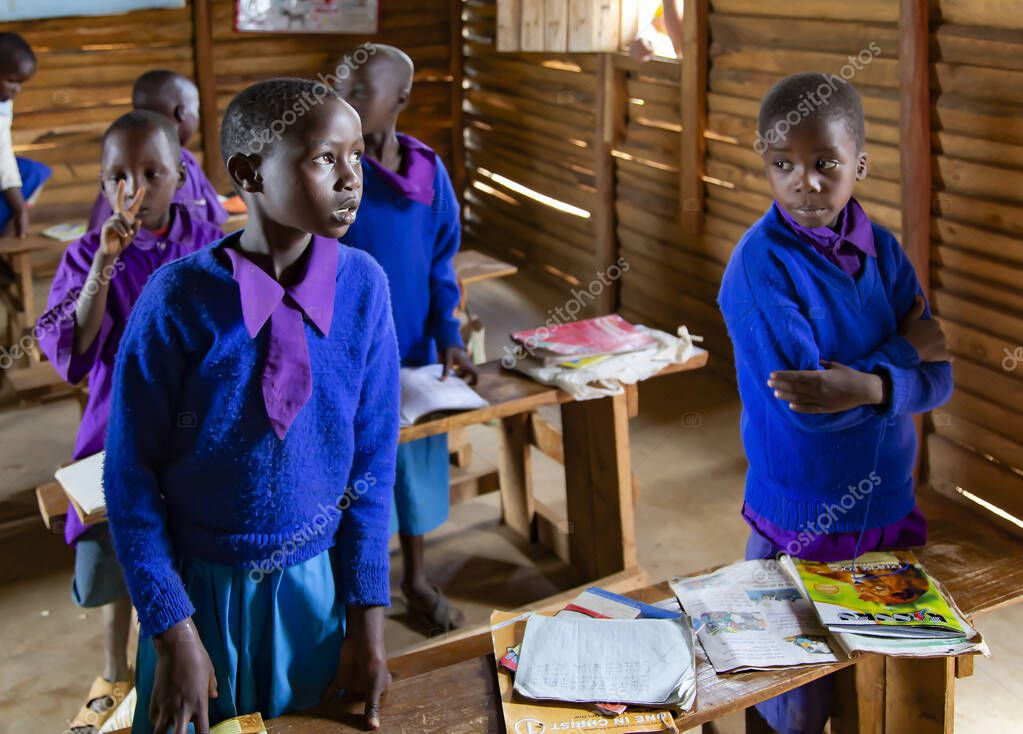
\includegraphics[width=\linewidth]{../Figures/deworming_children.jpg}
        \tiny{\centering \textit{Fuente: World Concern}}
    \end{column}
    \begin{column}{0.5\textwidth}
        \begin{itemize}
        \item \textbf{Desparasitación escolar} reduce infecciones intestinales.
        \item Mejora la salud general de los niños tratados y de sus compañeros no tratados.
        \item Aumenta la asistencia escolar al reducir el ausentismo por enfermedad.
        \item Mayor tiempo en la escuela fomenta mejores hábitos de salud y aprendizaje.
        \item Se generan \textbf{externalidades positivas} en la comunidad.
        \end{itemize}
    \end{column}
    \end{columns}
\end{frame}

\begin{frame}{Externalidades}
    \begin{itemize}
        \item Sucede cuando una decisión económica genera un beneficio o costo \textbf{externo}
        \item Afecta a terceros que no son capaces de internalizar estos beneficios o costos
        \item \textcolor{blue}{La clave es que estos beneficios o costos \textbf{¡no se reflejan en los precios!}}
        \begin{boxB}
            \centering
            Una externalidad sucede cuando el efecto de una decisión económica genera un beneficio (o un costo) a un tercero sin que este pague o tenga que pagar por él
        \end{boxB}
        \item Dos tipos de externalidades: 
        \begin{itemize}
            \item Externalidades negativas
            \item Externalidades positivas
        \end{itemize}
    \end{itemize}
\end{frame}

% \begin{frame}{Un ejemplo}
%     \centering
%     \href{https://econ.video/2022/06/20/the-g-word-with-adam-conover-externalities-regulation/}{
\includegraphics[scale=0.35]{../Figures/ExternalidadP.png}}  
% \end{frame}

\begin{frame}{Externalidades}
    \small
    \begin{columns}
        \begin{column}{0.5\textwidth}    
            \begin{figure} [H]
            \centering
            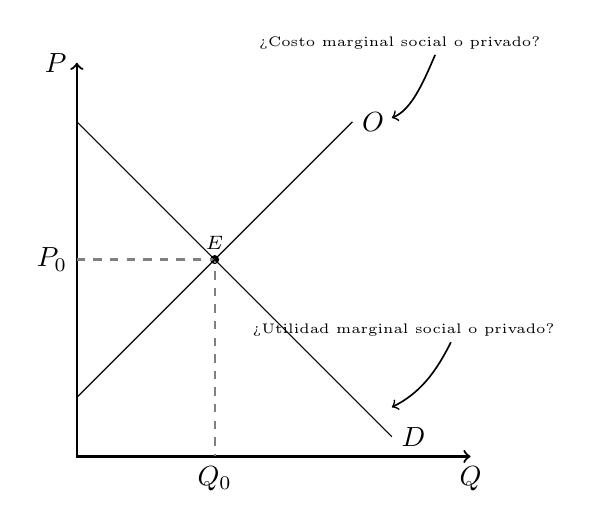
\begin{tikzpicture}[scale=0.5]
            
            \draw[thick,<->] (0,10) node[left]{$P$}--(0,0)--(10,0) node[below]{$Q$};
            
            \node [below] at (3.5,0) {{$Q_0$}};
            \draw[fill] (3.5,5) circle [radius =0.1] node[above] {\scriptsize $E$};
            \node [left] at (0,5) {$P_0$};
            
            % Flecha a la curva de oferta
            \draw[<-, semithick] (8,8.6)..controls (8.5,8.8) and (8.8,9.5)..(9.1,10.2);
            \node at (8.2,10.5) {\tiny ¿Costo marginal social o privado?};

            % Flecha a la curva de demanda
            \draw[<-, semithick] (8,1.25)..controls (8.7,1.6) and (9.1,2.1)..(9.5,2.9);
            \node at (8.3,3.2) {\tiny ¿Utilidad marginal social o privado?};

            \draw[thick,gray, dashed](0,5)--(3.5,5)--(3.5,0);
            \draw[thin](0,8.5)--(8,0.5) node[right] {$D$};
            \draw[black, domain=0:7] plot (\x, {1.5+\x}) node[right] {$O$};
            \end{tikzpicture}
            \end{figure} 
        \end{column}
        \begin{column}{0.5\textwidth}
            \begin{itemize}
                \item Las curvas siempre fueron \textbf{sociales}, aun que las veíamos como privadas.
                \item Si las curvas \textit{sociales} son diferentes a las \textit{privadas}, entonces hay una externalidad.
                \item ¿Que pasa con las cantidades de equilibrio?
                \item ¿Como afecta esto a productores y consumidores?
                \item ¿Como es la perdida o ganancia social?
            \end{itemize}
        \end{column}
    \end{columns}
\end{frame}

\begin{frame}{Tipos de externalidades}
    \small
    \begin{itemize}
        \item Se clasifican según:
        \begin{itemize}
            \item Si ocurren en el consumo o en la producción
            \item Si el efecto es negativo (daño) o positivo (beneficio)
        \end{itemize}
    \end{itemize}

    \vspace{0.3cm}
    \begin{table}[]
    \centering
    \scriptsize
    \begin{tabular}{|p{2.5cm}|p{2cm}|p{2.5cm}|p{3cm}|}
        \hline
        \textbf{Tipo de externalidad} & \textbf{Curva afectada} & \textbf{Desplazamiento} & \textbf{Ejemplo típico} \\
        \hline
        Negativa en producción  & Oferta  & Hacia arriba (\( \uparrow \)) & Contaminación industrial \\
        \hline
        Negativa en consumo     & Demanda & Hacia abajo (\( \downarrow \)) & Fumar en espacios cerrados \\
        \hline
        Positiva en producción  & Oferta  & Hacia abajo (\( \downarrow \)) & Apicultura que mejora cultivos vecinos \\
        \hline
        Positiva en consumo     & Demanda & Hacia arriba (\( \uparrow \)) & Vacunación, educación \\
        \hline
    \end{tabular}
    \end{table}
\end{frame}


\begin{frame}{Externalidades negativas}
    \begin{boxA}
        \centering
        Las externalidades negativas tienen lugar cuando el efecto de
        una decisión de producción, consumo u otro tipo de decisión
        económica de un agente genera un costo a un tercero que no es
        $\underline{\text{internalizado}}$ por quien lo produce.
    \end{boxA}
    \begin{itemize}
        \item La contaminación es un ejemplo clásico de externalidades negativas.
        \item El productor contaminante \textbf{no paga} por el costo extra que le está imponiendo a otros.
        \item Como no internaliza el costo ``total'' de su producción, produce más de lo que sería socialmente deseable.
        \item Para modelarlo, diferenciaremos entre costos marginales \textbf{privados} y costos marginales \textbf{sociales}.
    \end{itemize}
\end{frame}

\begin{frame}{Externalidades negativas}
    \begin{center}
        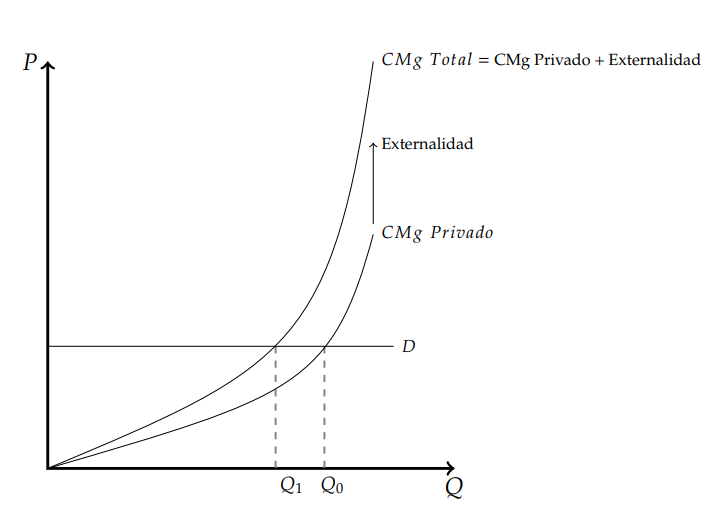
\includegraphics[scale=0.7]{../Figures/C25.2.png}
    \end{center}
\end{frame}

\begin{frame}{Externalidades negativas}
    \begin{figure} [H]
\centering
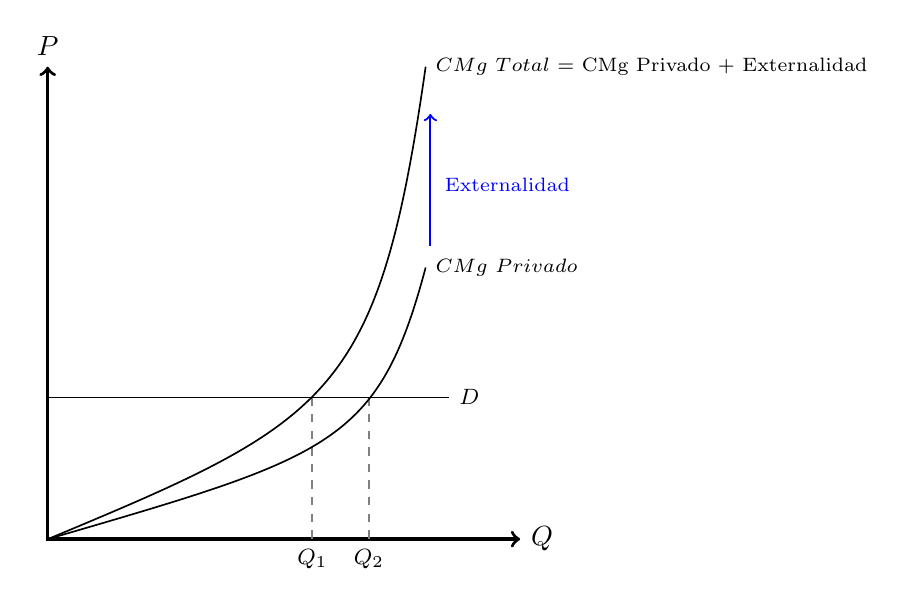
\begin{tikzpicture}[scale=0.6]
\draw[very thick,<->] (0,10) node[above]{$P$}--(0,0)--(10,0) node[right]{$Q$};
\draw[thick, dashed, gray] (5.6,3)--(5.6,0);
\draw[thick, dashed, gray] (6.8,3)--(6.8,0);
\draw [semithick] (0,0)..controls (6,1.75) and (7,2) .. (8,5.75) node [right] {\scriptsize $CMg \hspace{0.1cm} Privado$};
%\draw [semithick] (0 ,0)..controls (6,0.75) and (7,1) .. (8,4.75) node [right] {\scriptsize $Externalidad$};
\draw [semithick] (0,0)..controls (6,2.5) and (7,3) .. (8,10) node [right] {\scriptsize $CMg \hspace{0.1cm} Total$ = CMg Privado + Externalidad};
\draw[thick, ->, blue] (8.1,6.2) -- (8.1,9);
\node[right, blue] at (8.2,7.5) {\scriptsize Externalidad};
\draw[semithick] (0,3)--(8.5,3) node[right] {\footnotesize $D$};
\node[below] at (5.6,0) {\footnotesize $Q_1$};
\node[below] at (6.8,0) {\footnotesize $Q_2$};
\end{tikzpicture}
\end{figure} 
\end{frame}

\begin{frame}{¿Como corregir una externalidad negativa?}
    \begin{itemize}
        \item ¿Prohibir?
        \item ¿Regular la producción o el uso del contaminante?
        \item ¿Gravar (con un impuesto) la actividad contaminante?
        \item ¿Negociación privada?
    \end{itemize}
\end{frame}

\begin{frame}{Externalidad positiva}
    \begin{boxA}
        Las externalidades positivas tienen lugar cuando el efecto de
        toda decisión de producción, consumo u otro tipo de decisión
        económica de un agente genera un beneficio sobre un tercero sin
        que este pague por él.
    \end{boxA}
    \begin{itemize}
        \item La educación es un ejemplo clásico de externalidades positivas.
        \item El individuo que se educa recibe un beneficio, pero también lo recibe la sociedad.
        \item El individuo no recibe el beneficio total de su educación, por lo que no se educa lo suficiente.
        \item Para modelarlo, diferenciaremos entre beneficios marginales \textbf{privados} y beneficios marginales \textbf{sociales}.
    \end{itemize}
\end{frame}

% \begin{frame}{Otro ejemplo}
%     \centering  
%     \href{https://econ.video/2022/06/21/the-g-word-with-adam-conover-external-benefits-of-gps/}{
\includegraphics[scale=0.25]{../Figures/ExternalidadPII.png}}  
% \end{frame}


\begin{frame}{Externalidades positivas}
\begin{figure} [H]
\centering
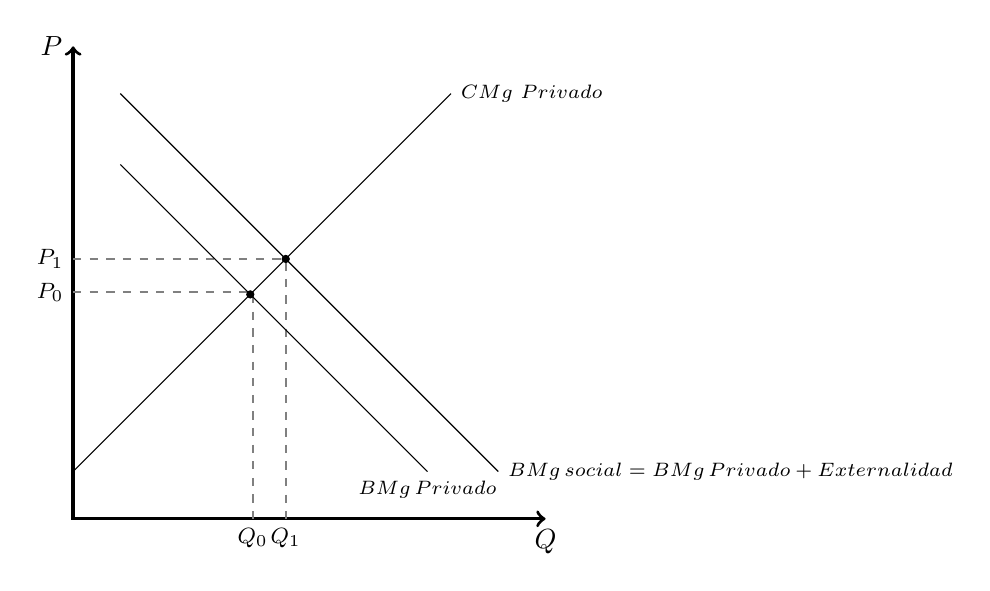
\begin{tikzpicture}[scale=0.6]
\draw[very thick,<->] (0,10) node[left]{$P$}--(0,0)--(10,0) node[below]{$Q$};
\draw[thick, dashed, gray] (0,4.8)--(3.8,4.8)--(3.8,0);
\draw[thick, dashed, gray] (0,5.5)--(4.5,5.5)--(4.5,0);
%\draw [thin] (0,0)..controls (6,1.75) and (7,2) .. (8,5.75) node [right] {\scriptsize $CMg \hspace{0.1cm} Privado$};
\draw [thin] (0,1)--(8,9) node [right] {\scriptsize $CMg \hspace{0.1cm} Privado$};
\draw[thin] (1,9)--(9,1) node [right] {\scriptsize $BMg \hspace{0.05cm} social = BMg \hspace{0.05cm} Privado  + Externalidad$};
\draw[thin] (1,7.5)--(7.5,1) node [below] {\scriptsize $BMg \hspace{0.05cm} Privado$};
\node[below] at (3.8,0) {\footnotesize $Q_0$};
\node[below] at (4.5,0) {\footnotesize $Q_1$};
\node[left] at (0,4.8) {\footnotesize $P_0$};
\node[left] at (0,5.5) {\footnotesize $P_1$};
\fill (3.75,4.75) circle (2.5pt);
\fill (4.5,5.5) circle (2.5pt);

\end{tikzpicture}
\end{figure} 
\end{frame}

\begin{frame}{¿Qué hacer con las externalidades positivas?}
    \begin{itemize}
        \item ¿Obligar?
        \item ¿Subsidiar su consumo?
    \end{itemize}
\end{frame}

\begin{frame}{Teorema de Coase}
    \begin{itemize}
        \item Coase dice que las externalidades no son un problema
        \item .... si los derechos de propiedad están bien definidos y los costos de transacción son nulos.
        \item Esto es así porque ``hay una ganancia para apropiar'' de buscar un óptimo.
    \end{itemize}
        \begin{boxB}
        \centering
        El \textbf{Teorema de Coase} señala que, en ausencia de costos de transacción y con derechos de propiedad bien definidos, una \textbf{negociación entre las partes }puede resultar en una asignación de recursos Pareto Eficiente, sin necesidad de la intervención del Estado
        \end{boxB}
\end{frame}

\begin{frame}{Curtiembres vs Pescadores I}
\begin{itemize}
    \item Supongamos que la producción de cueros genera una externalidad negativa en la producción de peces (la curtiembre tira químicos al río) \vspace{1mm}
    \item Como vimos, esto genera un costo marginal total que incluye el costo marginal privado y el costo de la externalidad.\vspace{1mm}
    \item ¿Cómo funcionaría el Teorema de Coase? Depende de cómo estén asignados los derechos de propiedad.
    \vspace{1mm}
    \item Caso I - Las curtiembres tienen derecho a contaminar:
    \begin{itemize}
        \item Cuando se produce $Q_0$, la pérdida de los pescadores es el \textcolor{blue!50}{área azul}.  
        \item Si quisieramos que la curtiembre produzca $Q_1$, habría que compensar su pérdida \textcolor{OrangeRed}{(área rayada rosa)}.
        \item ¿Se podría negociar? Sí! Porque la ganancia de los pescadores si se pasa a producir $Q_1$ es mayor a la pérdida de las curtiembres. 
        \item \textbf{Existe una negociación entre las partes que le permite a ambas llegar al óptimo}: al compensarlas, las curtiembres  ganan lo mismo  y los pescadores ganarían la diferencia entre el área azul y la rayada.
    \end{itemize}
\end{itemize}
\end{frame}


\begin{frame}{Coase I}
\begin{figure} [H]
\centering
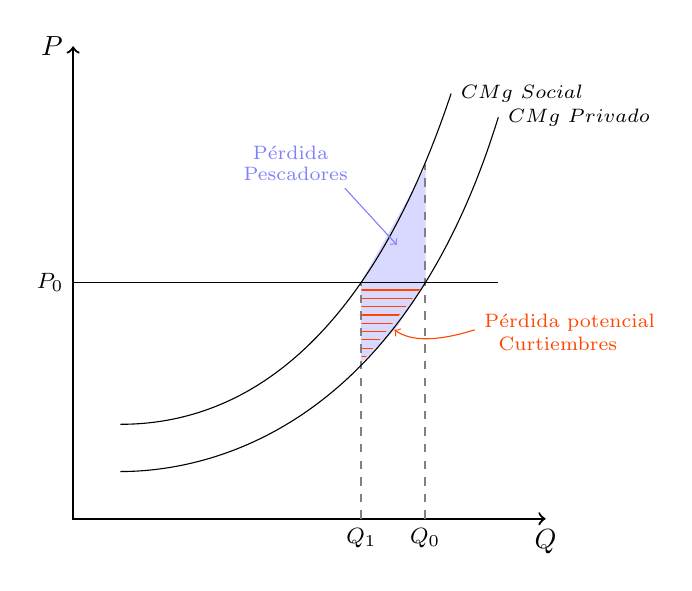
\begin{tikzpicture}[scale=0.6]
\draw[thick,<->] (0,10) node[left]{$P$}--(0,0)--(10,0) node[below]{$Q$};
\draw[fill,blue!15] (6.1,3.3)--(6.1,5)--(7.45,7.4)--(7.45,5)--(6.8,4);
% \draw[lines] (6.1,3.3)--(6.1,5)--(7.45,5)--(6.8,4);
% \draw[pattern=north west lines, pattern color=gray,solid] (6.1,3.3)--(6.1,5)--(7.45,5);
\path[pattern=horizontal lines,pattern color=OrangeRed] (6.1,3.3)--(6.1,5)--(7.45,5);
\draw[thick, gray,dashed] (7.45,0)--(7.45,7.5);
\draw[thick, gray,dashed] (6.1,0)--(6.1,5);
\draw [thin] (0,5) to (9,5) ;
\draw[thin] (1,2)..controls (3,2) and (6,3) .. (8,9) node [right] {\scriptsize $CMg \hspace{0.1cm} Social$};
\draw[thin] (1,1)..controls (3,1) and (7,2) .. (9,8.5) node [right] {\scriptsize $CMg \hspace{0.1cm} Privado$};
\node[left] at (0,5) {\footnotesize $P_0$};
\node[below] at (7.45,0) {\footnotesize $Q_0$};
\node[below] at (6.1,0) {\footnotesize $Q_1$};
\draw[thin, <-, OrangeRed] (6.8,4).. controls (7.15,3.75) and (7.7,3.75) ..(8.5,4);
\node [right, OrangeRed] at (8.5,4.15) {\scriptsize Pérdida potencial};
\node [right, OrangeRed] at (8.8,3.7) {\scriptsize Curtiembres};
\draw[thin, <-, blue!50] (6.85,5.8)--(5.75,7);
\node [right, blue!50] at (3.6,7.75) {\scriptsize Pérdida};
\node [right, blue!50] at (3.4,7.3) {\scriptsize Pescadores};
\end{tikzpicture}
\end{figure} 

\end{frame}

\begin{frame}{Curtiembres vs Pescadores II}
\begin{itemize}
    \item Caso II - Supongamos que son los pescadores los que tienen derecho al agua limpia. \vspace{1mm}
    \item ¿Cómo funcionaría ahora la negociación? 
    \begin{itemize}
        \item  La ganancia de las curtiembres por utilizar sus químicos hasta $Q_1$ es el \textcolor{blue!50}{área azul}.  
        \item Y la pérdida de los pescadores es el \textcolor{OrangeRed}{(área rayada rosa)}, que representa la externalidad negativa al producir $Q_1$.
        \item Si las curtiembres compensan a los pescadores por ese costo, la negociación nos lleva a un óptimo.
        \vspace{0.5mm}
        \item Es importante destacar que la mejor alternativa de compensación para la curtiembre se da en el punto $Q_1$.
        \begin{itemize}
        \item Si la curtiembre produce una unidad adicional, lo que gana marginalmente (línea azul) es menor a lo que debería pagarle a los pescadores para compensarlos por su pérdida (línea roja).
        \item Así, no sería negocio para las curtiembres compensar a los pescadores para producir por encima de $Q_1$.
        \end{itemize}
    \end{itemize}
\end{itemize}
\end{frame}

 
\begin{frame}{Coase II}
\begin{figure} [H]
\centering
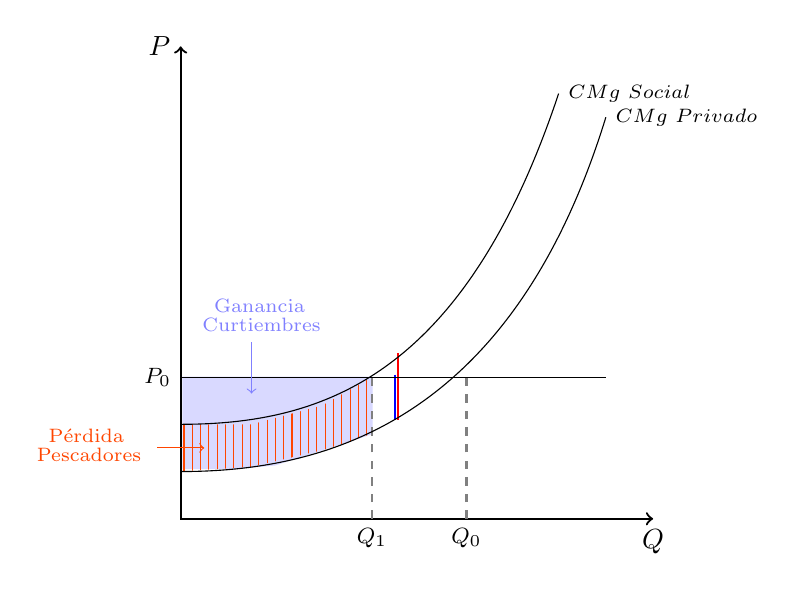
\begin{tikzpicture}[scale=0.6]
\draw[thick,<->] (0,10) node[left]{$P$}--(0,0)--(10,0) node[below]{$Q$};
\draw[fill,blue!15] (0.05,1.05)--(0.05,3)--(4.05,3)--(4.05,1.8)--(2,1.14)--(1,1.05);
\path[pattern=vertical lines,pattern color=OrangeRed] (0,1)--(0,2)--(1.5,2)--(3,2.4)--(4.05,3)--(4.05,1.8)--(3,1.45)--(1.5,1.1);
\draw[thick, gray,dashed] (4.05,0)--(4.05,3);
\draw[thick, gray,dashed] (6.05,0)--(6.05,3);
\draw[thick, red] (4.6,3.5)--(4.6,2.1);
\draw[thick, blue] (4.54,3.05)--(4.54,2.1);
\draw [thin] (0,3) to (9,3) ;
\draw[thin] (0,2)..controls (3,2) and (6,3) .. (8,9) node [right] {\scriptsize $CMg \hspace{0.1cm} Social$};
\draw[thin] (0,1)..controls (3,1) and (7,2) .. (9,8.5) node [right] {\scriptsize $CMg \hspace{0.1cm} Privado$};
\node[left] at (0,3) {\footnotesize $P_0$};
\node[below] at (4.05,0) {\footnotesize $Q_1$};
\node[below] at (6.05,0) {\footnotesize $Q_0$};
\draw[thin, ->, OrangeRed] (-0.5,1.5)--(0.5,1.5);
\draw[thin, <-, blue!50] (1.5,2.65)--(1.5,3.75);   
\node [right, blue!50] at (0.5,4.5) {\scriptsize Ganancia };
\node [right, blue!50] at (0.25,4.1) {\scriptsize Curtiembres};
\node [right, OrangeRed] at (-3,1.75) {\scriptsize Pérdida };
\node [right, OrangeRed] at (-3.25,1.35) {\scriptsize Pescadores};
\end{tikzpicture}
\end{figure} 
\end{frame}

\begin{frame}{Distorsiones al equilibrio de mercado}
    \begin{itemize}
        \item Por las características de la realidad: \vspace{1mm}
        \begin{itemize}
            \item Monopolios naturales (red eléctrica, agua, gas)   
             \vspace{1mm}
            \item Externalidades
             \vspace{1mm}
            \item \textbf{Bienes públicos}
            \vspace{1mm}
            \item Problemas de información
            \begin{itemize}
                \item Atributos ocultos (selección adversa)
                 \vspace{1mm}
                \item Acciones ocultas (moral hazard)
            \end{itemize}        
        \end{itemize}
    \end{itemize}
\end{frame}

\begin{frame}{Bienes Públicos}
    \begin{itemize}
        \item Vamos a distinguir los bienes por dos características:
        \begin{itemize}
            \item Si su consumo es rival: ¿el consumo de un individuo impide que otro lo consuma?
            \item Si su consumo es excluible: ¿es posible impedir que alguien consuma el bien en base a algún criterio?
        \end{itemize}
        \item Estas características hacen que los bienes divergan de los que conocemos como \textbf{bienes privados}.
        \item Los bienes públicos son no rivales y no excluibles: ¿Por qué no los puede ofrecer el mercado?
    \end{itemize}
    \begin{table}[]
        \centering
        \begin{tabular}{|>{\columncolor{blue!20}}c|c|c|}
        \hline
        \rowcolor{blue!20}
        & \textbf{Rival}   & \textbf{No rival} \\ \hline
        \textbf{Excluible} & \textbf{Bienes privados}  & Bienes club       \\ \hline
        \textbf{No Excluible} & Recursos comunes & \textbf{Bienes públicos}   \\ \hline
        \end{tabular}
    \end{table}
\end{frame}

\begin{frame}
\frametitle{El problema de los bienes públicos: el \textit{free-riding}}
        \begin{itemize}
            \item Como los bienes públicos son no rivales y no excluibles, las personas tienen incentivos a aprovechar el bien sin pagar por el mismo. 
            \vspace{1mm}
            \item Como nadie se encargaría de cubrir los costos, el mercado no puede ofrecer este tipo de bienes. Por eso, suelen ser provistos por el Estado.
            \vspace{1mm}
        \end{itemize}
        \begin{boxB}
        \centering
            El free-riding es el problema que surge cuando las personas tienen incentivos a utilizar un bien público sin contribuir en su producción, esperando que alguien más se encargue de cubrir los costos. Pero si todos piensan lo mismo, el bien termina por no producirse.
        \end{boxB}

\end{frame}

\begin{frame}
\frametitle{Intervención del Estado}
\begin{itemize}
\item Para la provisión de bienes públicos, decidir que el Estado intervenga es simplemente el primer paso. El gobierno debe entonces determinar qué tipo de bienes públicos ofrecer y en qué cantidades.
\item  Suponga que el gobierno está considerando construir una nueva autopista. Para evaluar su construcción, debe comparar los beneficios que obtendrían todos los usuarios de la autopista con los costos de construirla y darle mantenimiento. 
\item ¿Cómo cuantificar?
    \begin{itemize}
    \item Quienes usarán la autopista tienen un incentivo para exagerar el beneficio que obtendrán de la construcción de ésta.
    \item Quienes resulten perjudicados por la autopista tienen un incentivo para exagerar sus costos y evitar la construcción de la misma.
    \end{itemize}
\item La provisión eficiente de bienes públicos es entonces intrínsecamente más difícil que la provisión eficiente de bienes privados. 
\end{itemize}
\end{frame}

\begin{frame}{Bienes Club}
    \centering
    
\includegraphics[scale=0.12]{../Figures/M18.3.jpg}
    \hspace{15mm}
    
\includegraphics[scale=0.14]{../Figures/M18.4.png}
\end{frame}

\begin{frame}{Bienes Comunales}
    \begin{boxB}
        \centering
        La \textbf{tragedia de los comunes} describe la situación en la que los individuos acaban \textbf{sobreexplotando los recursos comunes} puesto que, como se trata de bienes rivales y no excluibles, tienen incentivos para utilizarlos antes que el resto.
    \end{boxB}
    \vspace{5mm}
    \centering
    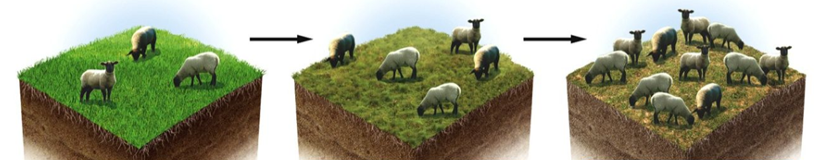
\includegraphics[scale=0.55]{../Figures/M18.5.png}
\end{frame}

\begin{frame}{Distorsiones al equilibrio de mercado}
    \begin{itemize}
        \item Por las características de la realidad: \vspace{1mm}
        \begin{itemize}
            \item Monopolios naturales (red eléctrica, agua, gas)   
             \vspace{1mm}
            \item Externalidades
             \vspace{1mm}
            \item Bienes públicos
            \vspace{1mm}
            \item \textbf{Problemas de información}
            \begin{itemize}
                \item Atributos ocultos (selección adversa)
                 \vspace{1mm}
                \item Acciones ocultas (moral hazard)
            \end{itemize}        
        \end{itemize}
    \end{itemize}
\end{frame}

\begin{frame}{Asimetrías de información}
    \begin{boxB}
        \centering
        \textbf{Hay información asimétrica cuando una de las partes tiene información de importancia para una transacción que la otra parte desconoce.}
    \end{boxB}
    \begin{itemize}
        \item Estos casos se enmarcan en el problema del \textbf{Principal-Agente}, donde el principal \textbf{contrata} a un agente para que realice una tarea.
        \item Pero el agente tiene información que el principal no tiene:
        \begin{itemize}
        \item Información de sus acciones $\rightarrow$ \textbf{Riesgo moral}
        \item Información de sus atributos $\rightarrow$ \textbf{Selección adversa}
        \end{itemize}
        \item Esto es mucho más común de lo que parece\dots
    \end{itemize}
\end{frame}

\begin{frame}{Selección Adversa}
    \begin{boxB}
        \centering
        La \textbf{selección adversa} es el problema que surge cuando una de las partes de una relación o intercambio no conoce ciertas características de la contraparte (\textbf{atributos ocultos}).
    \end{boxB}
    \vspace{2mm}
    \centering
    
\includegraphics[scale=0.5]{../Figures/M18.7.jpg} \hspace{2mm}
    
\includegraphics[scale=0.07]{../Figures/M18.6.png}
    \vspace{2mm}
    \begin{itemize}
        \item ¿Por qué las empresas te hacen exámenes antes de entrar?
        \item ¿Las prepagas pueden confiar en la salud de los nuevos clientes?
        \item ¿Los perfiles de Tinder muestran la verdad?
    \end{itemize}
\end{frame}

\begin{frame}{Selección Adversa}
    \begin{itemize}
        \item Cuando hay selección adversa, el riesgo (al igual que vamos a ver en riesgo moral) es que el mercado desaparezca.
        \vspace{1mm}
        \item Veamos un ejemplo clásico: el mercado de los limones de Akerlof.
        \vspace{1mm}
        \item Hay dos tipos de autos: buenos y malos (limones)
        \begin{itemize}
            \item Para el vendedor el auto bueno vale $\$1000$ y el malo $\$500$.
            \item Para el comprador el auto bueno vale $\$1500$ y el malo $\$750$.
        \end{itemize}
        \item ¿Cuanto está dispuesto a pagar un comprador? ¿Qué hace el vendedor?
        \item Si el comprador piensa que la probabilidad que un auto sea bueno es $\mu$ y que sea malo  $(1-\mu)$, el \textbf{valor esperado} para un auto típico en el mercado sería:
        \[\mu 1500 + (1-\mu) 750= 750 + \mu 750\] 
    \end{itemize}
\end{frame}

\begin{frame}{Selección Adversa: Los limones de Akerlof}

    \centering
    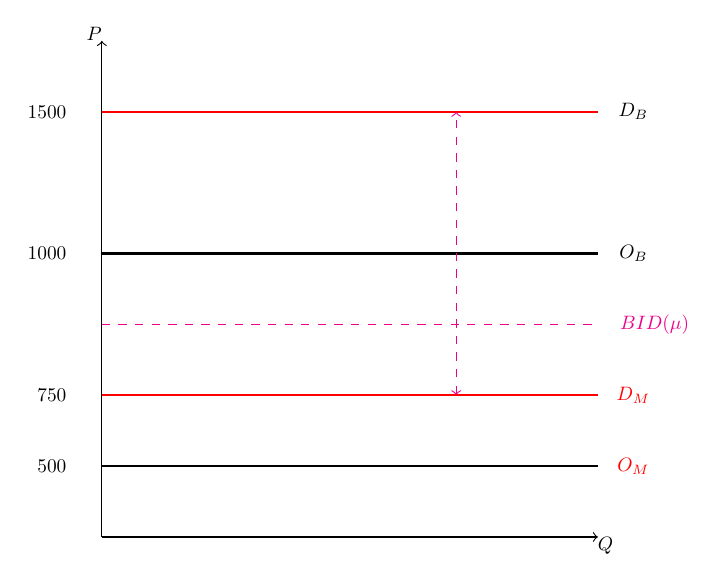
\begin{tikzpicture}[scale=0.9,every node/.style={scale=0.7, inner sep=0, outer sep=0}]

        % Coordenadas de los ejes
        \draw[->, black] (0, 0) -- (7, 0) node[below right] {$Q$}; % Eje x
        \draw[->, black] (0, 0) -- (0, 7) node[above left] {$P$};  % Eje y
        
        % Números de valores en y
        \node[black, anchor=east] at (-0.5, 6) {1500};
        \node[black, anchor=east] at (-0.5, 4) {1000};
        \node[black, anchor=east] at (-0.5, 2) {750};
        \node[black, anchor=east] at (-0.5, 1) {500};
    
        
        % Líneas horizontales
        \draw[thick, black] (0, 1) -- (7, 1);
        \draw[thick, red] (0, 2) -- (7, 2);
        \draw[dashed, magenta] (0, 3) -- (7, 3);
        \draw[thick, black] (0, 4) -- (7, 4);
        \draw[thick, red] (0, 6) -- (7, 6);
        
        % Flecha vertical magenta entre las líneas rosas
        \draw[dashed, magenta, <->] (5, 2) -- (5, 6);
        
        % Textos
        \node[red] at (7.5, 2) {$D_M$};
        \node[red] at (7.5, 1) {$O_M$};
        \node[magenta] at (7.8, 3) {$BID (\mu)$};
        \node[black] at (7.5, 4) {$O_B$};
        \node[black] at (7.5, 6) {$D_B$};
        
    \end{tikzpicture}
\end{frame}

\begin{frame}{Selección Adversa: Los limones de Akerlof}
    \begin{itemize}
    \item El vendedor venderá un auto si lo que pide por él es menor a lo que el consumidor valora el auto en términos esperados.
    \vspace{1mm}
    \item Si tiene un lemon, esto sucede si: $500\leq750+\mu750$
        \begin{itemize}
        \item Osea, si el vendedor tiene un auto malo, lo pone en el mercado siempre! 
        \end{itemize}
    \vspace{1mm}
    \item Si tiene un auto bueno, lo venderá si: 
    $1000 \leq 750 + \mu 750 $ 
        \begin{itemize}
        \item Esto solo se daría si $\mu \geq \frac{1}{3}$
        \end{itemize} 
    \item  Si hay suficiente autos buenos en el mercado, hay un equilibrio donde $\mu \geq \frac{1}{3}$ y $p= 750 + \mu 750$ y se venden los dos tipos de autos.     \vspace{1mm}
    \item Pero si hay pocos autos buenos, los compradores saben que la probabilidad de que sea bueno es muy chica.
    \begin{itemize}
    \item El vendedor no ofrecerá autos nuevos, ya que no los vendería
    \item Si $q= \mu = 0 $, se venden solo lemons y el precio de venta es $p= 750$ 
    \end{itemize}
    \item El mercado para autos buenos desapareció aun cuando dijimos al principio que estos tenían más valor para los consumidores que para los vendedores. 
    \end{itemize}   
\end{frame}

\begin{frame}{Riesgo Moral}
    \begin{boxB}
        \centering
        El \textbf{riesgo moral} es el problema que surge cuando no podemos ver el accionar de la contraparte (\textbf{acciones ocultas}).
    \end{boxB}
    \begin{itemize}
        \item Lo importante acá es que un Agente toma una decisión o realiza una acción que afecta su
        utilidad y la utilidad del Principal.
        \item ¿Contratos laborales atados a objetivos? ¿Pagos en acciones de la empresa?
        \item ¿Por qué los propietarios te piden una garantía para alquilar?
    \end{itemize}
    \centering
    % 
\includegraphics[scale=0.4]{../Figures/FMI_Riesgo_Moral.jpg}
\end{frame}


\begin{frame}{Ejemplos}
    \begin{itemize}
    \item \href{https://www.youtube.com/watch?v=qlg0qakJhKU}{\textbf{Matilda}}
    \item \href{https://www.youtube.com/watch?v=akA8co61He4}{\textbf{Tomates verdes fritos}}
    \item \href{https://www.youtube.com/watch?v=X8BPfLhH6MA}{\textbf{Friends}}
    \item \href{https://videos.criticalcommons.org/media/encoded/16/jtierney86/43ba1b1ac3e94df3974f987cc912ae_Hxgbfl1.mp4}{\textbf{The Daily Show}}
    \item \href{http://videos.criticalcommons.org/transcoded/http/www.criticalcommons.org/Members/JJWooten/clips/always-sunny-paying-for-care/video_file/mp4-high/always-sunny-cost-of-care-mp4.mp4}{\textbf{Always sunny}}
    \item \href{https://www.youtube.com/watch?v=SrPu-xGrKrk}{\textbf{Buying a car}}
    \item \href{https://www.youtube.com/watch?v=ZZq0ShjEd-E}{\textbf{But he has a Bud Light}}
    \end{itemize}

\end{frame}


\begin{frame}{Riesgo moral y el colapso del mercado de seguros}
 \begin{itemize}
    \item Imaginemos una persona que tiene que comprar un seguro de incendio para su casa
    \begin{itemize}
    \item la casa puede no incendiarse y el individuo no pierde nada : Evento Bueno con probabilidad $p$
    \item la casa puede incendiarse y el individuo sufre una pérdida de tamaño $L$: Evento Malo con probabilidad $(1-p)$ 
    \end{itemize}
    \vspace{1mm}
    \item La probabilidad del evento bueno depende en parte de alguna acción del individuo, vamos a decir que depende del esfuerzo del individuo: $p(e)$
    \begin{itemize}
    \item Por ejemplo: el individuo esta alerta a no dejar electrodomésticos enchufados, ni hornallas encendidas, le hace mantenimiento al hagor, etc.
    \end{itemize}
    \item La clave es entender que quien ofrece el seguro no puede ver esta acción o esfuerzo
\end{itemize}
\end{frame}

\begin{frame}{Riesgo moral II}
    \begin{itemize}
    \item Si la compañía aseguradora ofrece una cobertura de valor $C$ a un precio $\pi C$ (el precio depende de la cobertura) \vspace{2mm}
    \item En el escenario bueno, la utilidad para el individuo es 
    $U_B = y - \pi C$
    \item Si se produce el evento malo, su utilidad para el individuo es 
    $U_M = y - L - \pi C + C$ \vspace{2mm}
    \item ¿Qué $\pi$ podría cobrar la compañía de seguros?
    \begin{itemize}
    \item La ecuación de ganancias de las aseguradoras es  
    $\pi C - (1-p) C$
    \item Si esta ganancia la hacemos $0$ el (menor) porcentaje que puede cobrar la compañía es $\pi=(1-p)$
    \end{itemize}
    \end{itemize}
\end{frame}

\begin{frame}{Riesgo moral III}
    \begin{itemize}
    \item Si el individuo compra una cobertura de $C=L$, es decir, se asegura totalmente:
    \begin{itemize}
    \item En el escenario bueno, la utilidad para el individuo es 
    $U_B = y - \pi L$
    \item Si se produce el evento malo, su utilidad para el individuo es 
    $U_M = y - L - \pi L + L = y - \pi L$ 
    \end{itemize}
    \item Le es indiferente si se produce el evento bueno o el malo 
    \item Pero entonces $e=0$, es decir, no va a esforzarse por cuidar la casa, y la probabilidad del evento malo va a ser más alta \vspace{2mm}
    \item Si el individuo no hace nada el siniestro ocurre con probabilidad $(1-p)=1$, y en este caso, $p=0$ y $\pi=1$
    \item La utilidad para el individuo de comprar seguro es $y-L$, que resulta peor que no comprar seguro $y$
    \item ¡Es decir que el mercado asegurador desaparece! 
  \end{itemize}   
\end{frame}


\begin{frame}{Discusiones}
    \begin{itemize}
        \item ¿Por qué pierden valor los autos al salir de la concesionaria? \vspace{1mm}
        \item Políticas de deducibles \vspace{1mm}
        \item Obama care
    \end{itemize}
\end{frame}

\end{document}
